\documentclass[../main.tex]{subfiles}

\makeatletter
\@ifundefined{fromRoot}{%
  \newcommand{\fromRoot}[1]{../#1}
  
  \usepackage{xr}
  \externaldocument{../main}
}{}

\def\input@path{{\subfix{../}}}
%or: \def\input@path{{/path/to/folder/}{/path/to/other/folder/}}
\makeatother

\graphicspath{
  {\subfix{../}}
  {\subfix{./figures}}
  {\subfix{../figures}}
  {\subfix{./figures/logos-thesis/}}
  {\subfix{../figures/logos-thesis/}}
  {\subfix{./figures/rtexps-pics/}}
  {\subfix{../figures/rtexps-pics/}}
}

\hypersetup{
    pdfauthor   = {Camille MONIÈRE},
    pdftitle    = {Th\`{e}se (Présentation: étude algorithmique)},
    pdfsubject  = {Th\`{e}se (Présentation: étude algorithmique)},
%    pdfkeywords = {mots-cl\'{e}s},
}

\begin{document}

\section{Étude algorithmique}

% \subsection{Sensibilité à un facteur d'échelle}


% \begin{frame}{\subsecname}
%   \begin{center}
%     \textcolor{RoyalBlue}{TODO}
%   \end{center}
% \end{frame}


\subsection{Corrélation glissante dans le temps (\emph{Time sliding})}

\begin{frame}{Criticité de la tache de corrélation}
  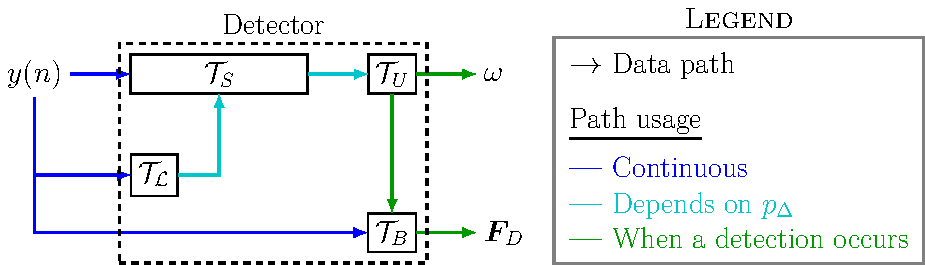
\includegraphics[width=\linewidth]{figures/tikzpicture/tasks_dep_stdl.pdf}
  \begin{center}
    \textcolor{RoyalBlue}{TODO}
  \end{center}
\end{frame}

\begin{frame}{Méthode par FFT}
  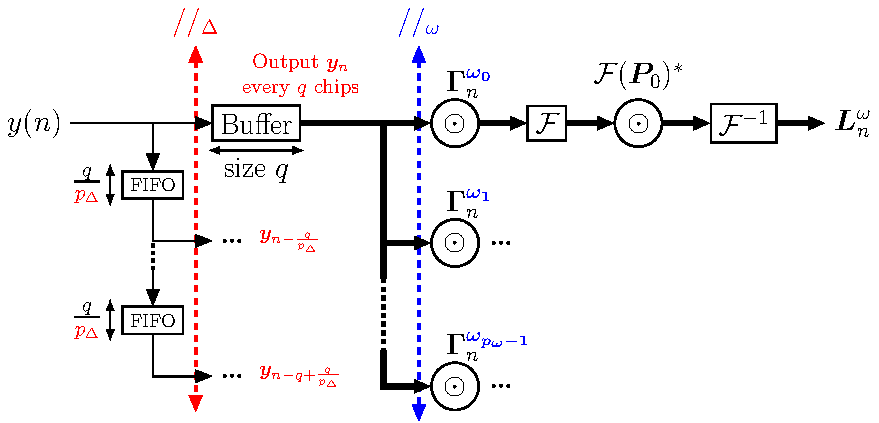
\includegraphics[width=\linewidth]{figures/tikzpicture/corr_method_fft_stdl.pdf}
  \begin{center}
    \textcolor{RoyalBlue}{TODO}
  \end{center}
\end{frame}

\begin{frame}{Méthode par TS Data shift}
  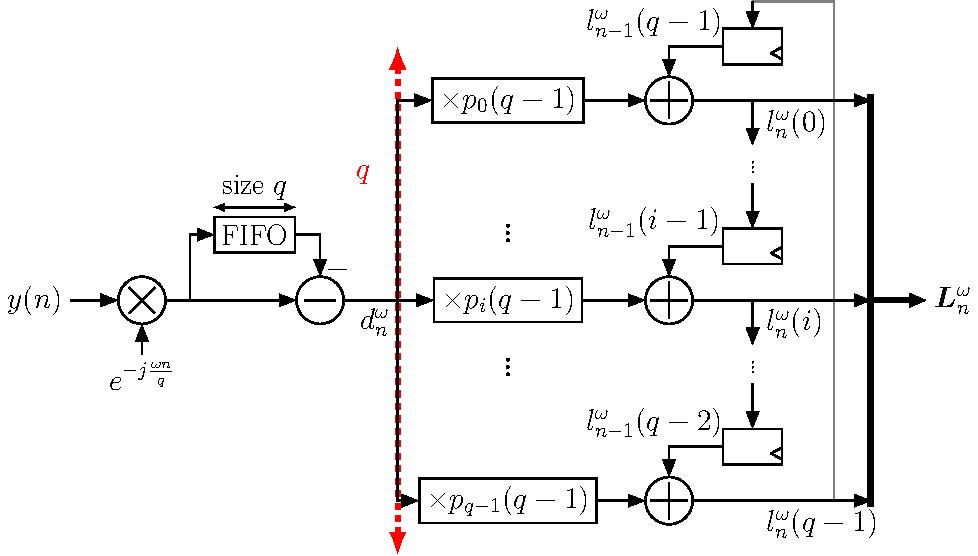
\includegraphics[width=\linewidth]{figures/tikzpicture/arch_statts_sync_stdl.pdf}
  \begin{center}
    \textcolor{RoyalBlue}{TODO}
  \end{center}
\end{frame}

\begin{frame}{Méthode par FFT}
  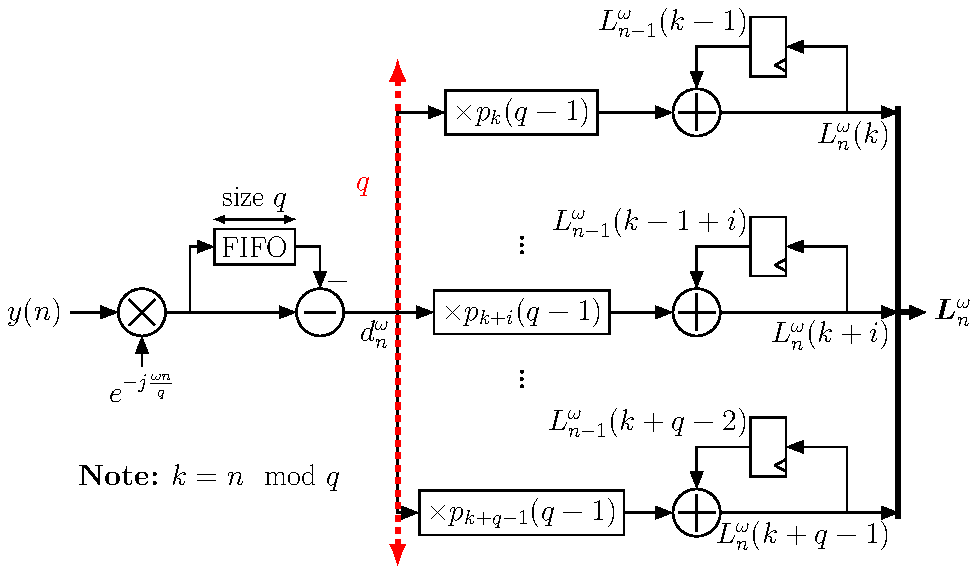
\includegraphics[width=\linewidth]{figures/tikzpicture/arch_subts_sync_stdl.pdf}
  \begin{center}
    \textcolor{RoyalBlue}{TODO}
  \end{center}
\end{frame}

\end{document}
